\documentclass[11pt,a4paper]{report}
\usepackage[english]{babel}
\usepackage[utf8]{inputenc}
\usepackage[T1]{fontenc}
\usepackage{glossaries}
\usepackage{graphicx}
\usepackage{hyperref}
\usepackage{wrapfig}
\usepackage{float}
\usepackage{natbib}
\usepackage{listings}
\usepackage{caption}
\usepackage{subcaption}

\usepackage{color}
 
\definecolor{codegreen}{rgb}{0,0.6,0}
\definecolor{codegray}{rgb}{0.5,0.5,0.5}
\definecolor{codepurple}{rgb}{0.58,0,0.82}
\definecolor{backcolour}{rgb}{0.95,0.95,0.92}

\graphicspath{ {images/} }

\newcommand{\HRule}{\rule{\linewidth}{0.5mm}}
\setlength\parindent{0pt} 

\let\olditemize\itemize
\renewcommand{\itemize}{
  \olditemize
  \setlength{\itemsep}{1pt}
  \setlength{\parskip}{0pt}
  \setlength{\parsep}{0pt}
}

\title{\textbf{Internet Service Provider ARA Project} \\Arquitectura de Redes Avançada \\Universidade de Aveiro}
\author{Diogo Silva 60337 \and Eduardo Sousa 68633 \and \\Docente: Prof. Paulo Salvador}

\begin{document}
\begin{titlepage}
\begin{center}
\HRule \\[0.4cm]
{ \huge \bfseries Internet Service Provider ARA Project \\[0.4cm] }
\HRule \\[1.5cm]
\textsc{\LARGE Universidade de Aveiro}\\[1.5cm]
\textsc{}\\[1.5cm]
\textsc{Diogo Silva 60337 \\Eduardo 68633 \\\hphantom \newline Docente: Prof. Paulo Salvador}
\end{center}
\end{titlepage}
\maketitle
\tableofcontents

\lstdefinestyle{mystyle}{
    backgroundcolor=\color{backcolour},   
    commentstyle=\color{codegreen},
    keywordstyle=\color{magenta},
    numberstyle=\tiny\color{codegray},
    stringstyle=\color{codepurple},
    basicstyle=\footnotesize,
    breakatwhitespace=false,         
    breaklines=true,                 
    captionpos=b,                    
    keepspaces=true,                 
    numbers=left,                    
    numbersep=5pt,                  
    showspaces=false,                
    showstringspaces=false,
    showtabs=false,                  
    tabsize=2
}
\lstset{style=mystyle}

\chapter{Basic Mechanisms and BGP}

\begin{figure}[H]
\centerline{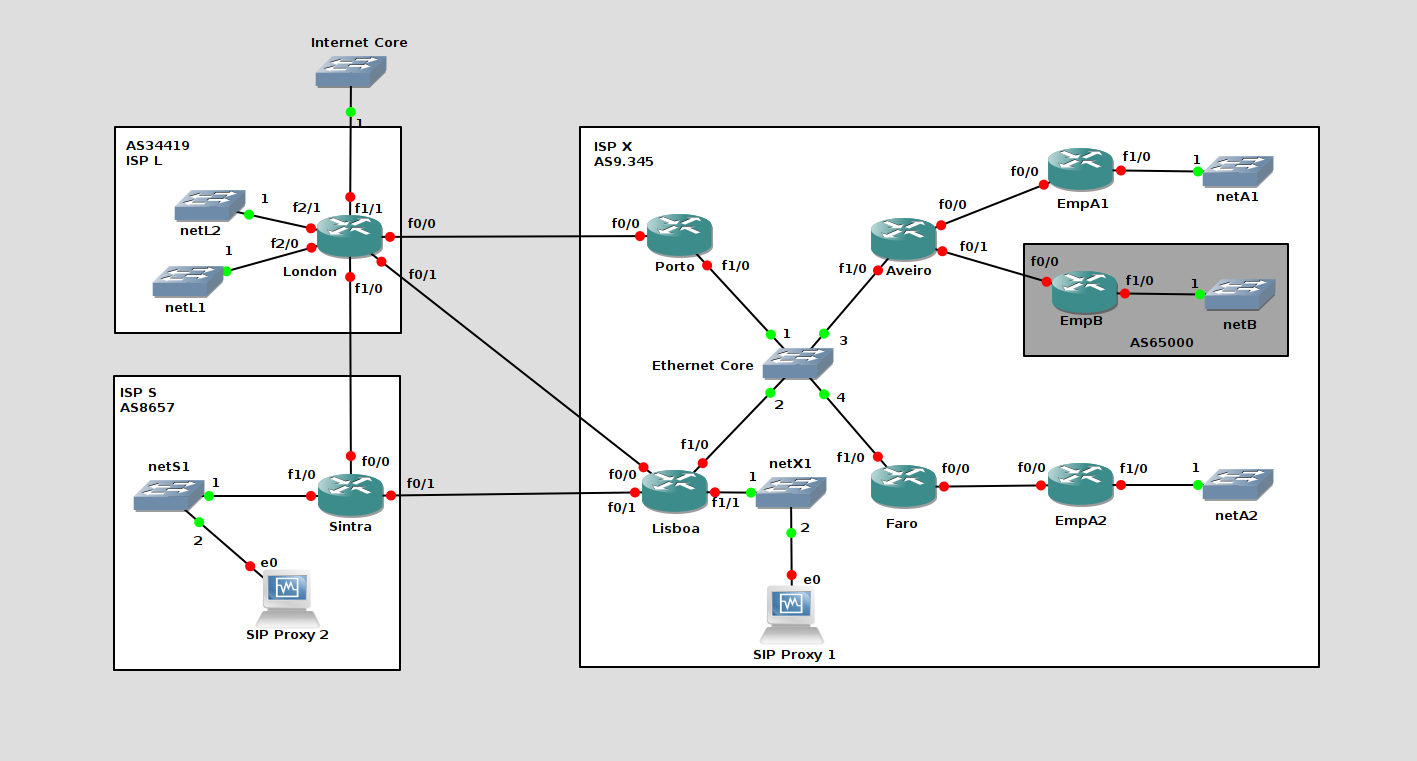
\includegraphics[scale=0.5]{network.png}}
\caption{Visão geral da rede}
\label{schema}
\end{figure}

\section{Internal BGP \& OSPF Redistribution}
Neste projeto foi necessário utilizar Internal BGP para ligar os routers do ethernet core do ISP X e o AS privado 65000 pertencente à empresa B. Isto permitiu que as redes públicas fossem anunciadas diretamente por BGP pela rede do ISP X e do AS privado 65000.\\
Foi necessário também utilizar OSPF para as redes internas, que foi redistribuido para o Internal BGP.\\
Os routers foram configurados da seguinte maneira:

\begin{lstlisting}[caption=Internal BGP - Router Porto]
router bgp 9.345
  address-family ipv4 unicast
  	network 192.172.100.0 mask 255.255.255.128
    neighbor 192.172.100.2 remote-as 590169
	neighbor 192.172.100.2 update-source Loopback0
 	neighbor 192.172.100.2 next-hop-self
 	neighbor 192.172.100.3 remote-as 590169
 	neighbor 192.172.100.3 update-source Loopback0
 	neighbor 192.172.100.3 next-hop-self
 	neighbor 192.172.100.4 remote-as 590169
 	neighbor 192.172.100.4 update-source Loopback0
  	neighbor 192.172.100.4 next-hop-self
  address-family ipv6 unicast
  	network 2001:192:100::/48
  	neighbor 2001:192:100::2 remote-as 590169
 	neighbor 2001:192:100::2 update-source Loopback0
 	neighbor 2001:192:100::2 next-hop-self
 	neighbor 2001:192:100::3 remote-as 590169
 	neighbor 2001:192:100::3 update-source Loopback0
 	neighbor 2001:192:100::3 next-hop-self
 	neighbor 2001:192:100::4 remote-as 590169
 	neighbor 2001:192:100::4 update-source Loopback0
 	neighbor 2001:192:100::4 next-hop-self
\end{lstlisting}

\begin{lstlisting}[caption=Internal BGP - Router Lisboa]
  	!route-map, eBGP, remove-private-as foi tudo omitido neste ponto
router bgp 9.345
  address-family ipv4 unicast
  	network 192.172.100.0 mask 255.255.255.128
  	network 192.172.100.128 mask 255.255.255.128
    neighbor 192.172.100.1 remote-as 590169
	neighbor 192.172.100.1 update-source Loopback0
 	neighbor 192.172.100.1 next-hop-self
 	neighbor 192.172.100.3 remote-as 590169
 	neighbor 192.172.100.3 update-source Loopback0
 	neighbor 192.172.100.3 next-hop-self
 	neighbor 192.172.100.4 remote-as 590169
 	neighbor 192.172.100.4 update-source Loopback0
  	neighbor 192.172.100.4 next-hop-self
  address-family ipv6 unicast
  	network 2001:192:100::/48
  	network 2001:192:101::/48
  	neighbor 2001:192:100::1 remote-as 590169
 	neighbor 2001:192:100::1 update-source Loopback0
 	neighbor 2001:192:100::1 next-hop-self
 	neighbor 2001:192:100::3 remote-as 590169
 	neighbor 2001:192:100::3 update-source Loopback0
 	neighbor 2001:192:100::3 next-hop-self
 	neighbor 2001:192:100::4 remote-as 590169
 	neighbor 2001:192:100::4 update-source Loopback0
 	neighbor 2001:192:100::4 next-hop-self
\end{lstlisting}

\begin{lstlisting}[caption=Internal BGP  \& OSPF Redistribute - Router Aveiro]
  	!route-map, eBGP, remove-private-as foi tudo omitido neste ponto
router bgp 9.345
  address-family ipv4 unicast
  	network 192.172.100.0 mask 255.255.255.128
  	redistribute static route-map rm-priv-default4
  	redistribute ospf 100 route-map rm-priv-default4
  	neighbor 10.1.100.10 remote-as 65000
    neighbor 192.172.100.1 remote-as 590169
	neighbor 192.172.100.1 update-source Loopback0
 	neighbor 192.172.100.1 next-hop-self
 	neighbor 192.172.100.2 remote-as 590169
 	neighbor 192.172.100.2 update-source Loopback0
 	neighbor 192.172.100.2 next-hop-self
 	neighbor 192.172.100.4 remote-as 590169
 	neighbor 192.172.100.4 update-source Loopback0
  	neighbor 192.172.100.4 next-hop-self
  	!route-map, eBGP, remove-private-as foi tudo omitido neste ponto
  address-family ipv6 unicast
  	network 2001:192:100::/48
  	redistribute ospf 200
  	neighbor 2001:192:100::B remote-as 65000
  	neighbor 2001:192:100::1 remote-as 590169
 	neighbor 2001:192:100::1 update-source Loopback0
 	neighbor 2001:192:100::1 next-hop-self
 	neighbor 2001:192:100::2 remote-as 590169
 	neighbor 2001:192:100::2 update-source Loopback0
 	neighbor 2001:192:100::2 next-hop-self
 	neighbor 2001:192:100::4 remote-as 590169
 	neighbor 2001:192:100::4 update-source Loopback0
 	neighbor 2001:192:100::4 next-hop-self
\end{lstlisting}

A configuração de Faro é bastante similar a de Aveiro:\\

\begin{lstlisting}[caption=Internal BGP  \& OSPF Redistribute - Router Faro]
  	!route-map, eBGP, remove-private-as foi tudo omitido neste ponto
router bgp 9.345
  address-family ipv4 unicast
  	network 192.172.100.0 mask 255.255.255.128
  	redistribute static route-map rm-priv-default4
  	redistribute ospf 100 route-map rm-priv-default4
    neighbor 192.172.100.1 remote-as 590169
	neighbor 192.172.100.1 update-source Loopback0
 	neighbor 192.172.100.2 remote-as 590169
 	neighbor 192.172.100.2 update-source Loopback0
 	neighbor 192.172.100.3 remote-as 590169
 	neighbor 192.172.100.3 update-source Loopback0
  address-family ipv6 unicast
  	network 2001:192:100::/48
  	redistribute ospf 300
  	neighbor 2001:192:100::1 remote-as 590169
 	neighbor 2001:192:100::1 update-source Loopback0
 	neighbor 2001:192:100::2 remote-as 590169
 	neighbor 2001:192:100::2 update-source Loopback0
 	neighbor 2001:192:100::3 remote-as 590169
 	neighbor 2001:192:100::3 update-source Loopback0
\end{lstlisting}

Nas configurações é possível ver ``update-source Loopback0'' que é o que permite estabelecer as ligações TCP das relação peer do BGP, sendo que a interface de Loopback 0 nunca vai abaixo é melhor ser definida sobre ela.\\

Para além disso também se usou ``next-hop-self'' quando se tinha uma relação de iBGP na fronteira do AS, porque era necessário mudar o atributo next-hop que o router de Lisboa e Porto recebiam das relação eBGP (de Sintra e London) para eles próprios, se não a rede de iBGP não conhecia o next-hop anunciado e ia falhar a comunicação.

Pode ser verificado nas imagens seguintes o funcionamento de Internal BGP.

\begin{figure}[H]
\centerline{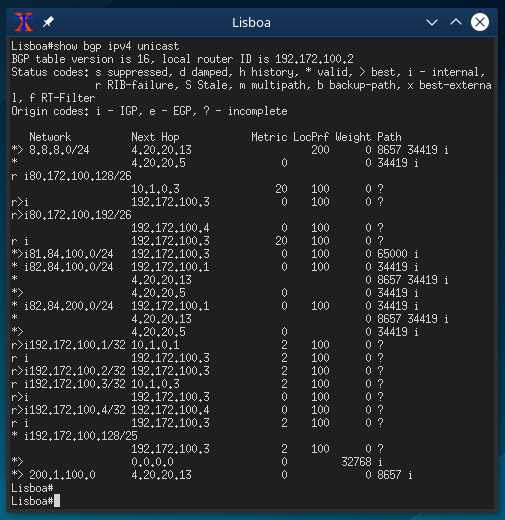
\includegraphics[width=260pt]{lisboa_bgp_ipv4.png}}
\caption{Tabelas de redes aprendidas por BGP e OSPF em IPv4}
\label{schema}
\end{figure}

\begin{figure}[H]
\centerline{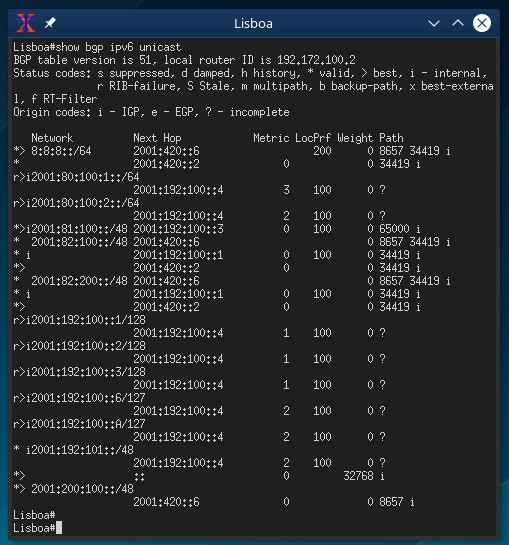
\includegraphics[width=260pt]{lisboa_bgp_ipv6.png}}
\caption{Tabelas de redes aprendidas por BGP e OSPF em IPv6}
\label{schema}
\end{figure}

\section{External BGP}
Foi necessário também estabelecer ligações BGP com outros AS de forma a termos acesso a outros serviços como por exemplo PTSN. As ligações estabelecidas foram com o AS8657 pertencente ao ISP S e com o AS 34419 pertencente ao ISP L. Ao serem estabelecidas estas ligações o ISP X passou a ter conetividade com o Internet Core bem como as redes pertencentes a esses AS. As seguintes configurações foram utilizadas.

\begin{lstlisting}[caption=External BGP - Router Porto]
router bgp 9.345
  address-family ipv4 unicast
  	neighbor 4.20.20.1 remote-as 34419
  address-family ipv6 unicast
  	neighbor 2001:420:: remote-as 34419
\end{lstlisting}

\begin{lstlisting}[caption=External BGP - Router Lisboa]
router bgp 9.345
  address-family ipv4 unicast
  	neighbor 4.20.20.5 remote-as 34419
	neighbor 4.20.20.13 remote-as 8657
  address-family ipv6 unicast
  	neighbor 2001:420::2 remote-as 34419
 	neighbor 2001:420::6 remote-as 8657
\end{lstlisting}

Através das configurações definidas anteriormente é possível verificar nas tabelas de redes aprendidas por BGP dos routers de Londres e Sintra que o External BGP se encontra bem configurado.

\begin{figure}[H]
\centerline{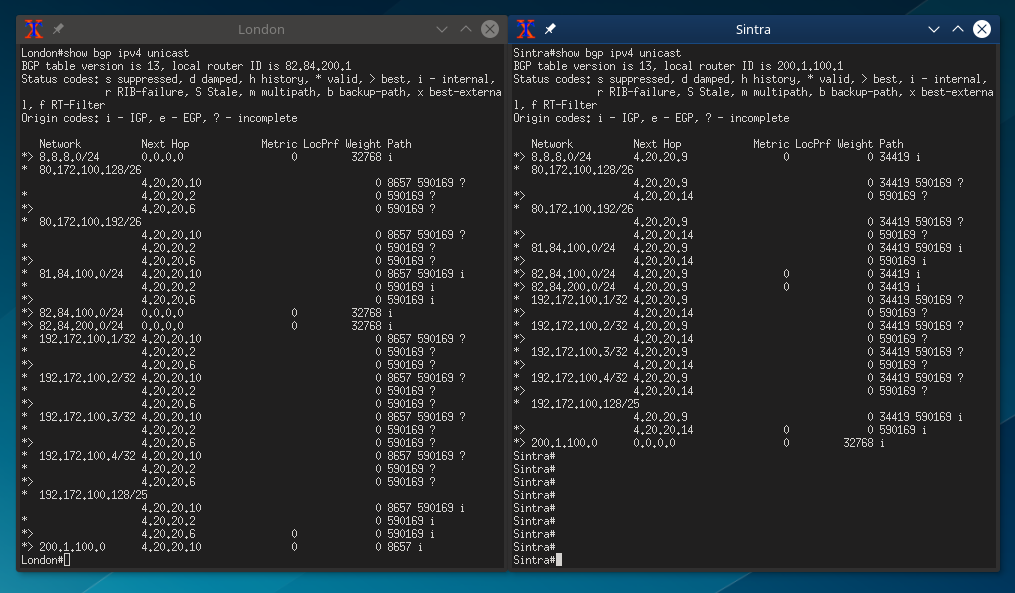
\includegraphics[width=300pt]{private_as_removal_ipv4.png}}
\caption{Tabelas de redes aprendidas por BGP em IPv4}
\label{schema}
\end{figure}

\begin{figure}[H]
\centerline{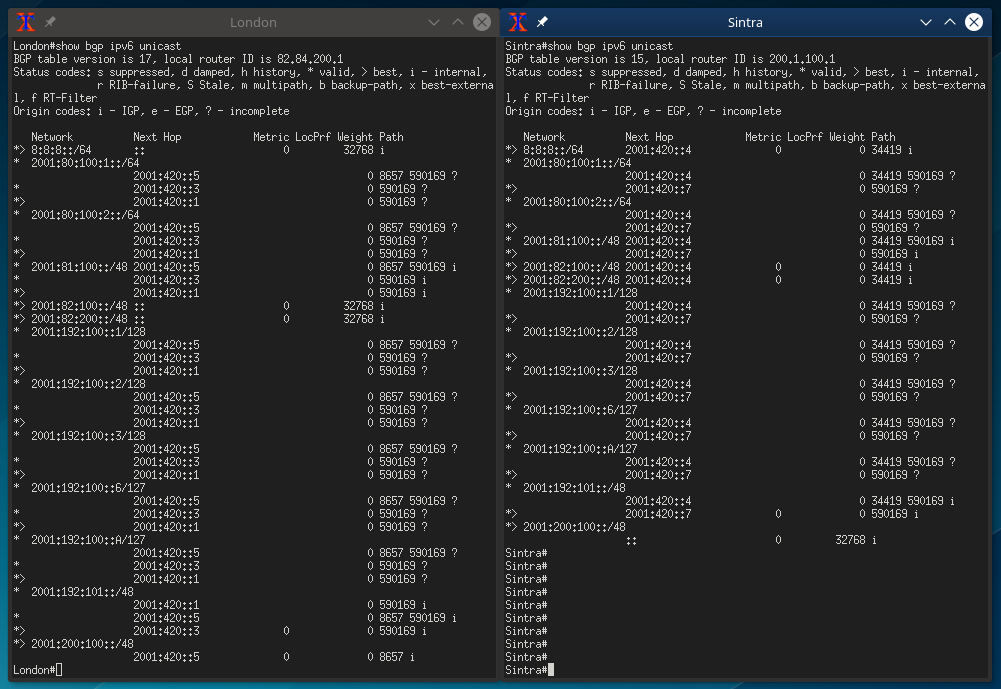
\includegraphics[width=300pt]{private_as_removal_ipv6.png}}
\caption{Tabelas de redes aprendidas por BGP em IPv6}
\label{schema}
\end{figure}

\section{Private AS}
Houve a necessidade de configurar um AS privado para a empresa B. Esse AS com o identificador 65000 é filtrado dos anuncios de BGP para os outros AS. A seguinte configuração foi efetuada nos routers do Porto e Lisboa:

\begin{lstlisting}[caption=Remoção do AS privado - Router Porto]
router bgp 9.345
  address-family ipv4 unicast
    neighbor 4.20.20.1 remove-private-as
  address-family ipv6 unicast
  	neighbor 2001:420:: remove-private-as
\end{lstlisting}

\begin{lstlisting}[caption=Remoção do AS privado - Router Lisboa]
router bgp 9.345
  address-family ipv4 unicast
    neighbor 4.20.20.5 remove-private-as
    neighbor 4.20.20.13 remove-private-as
  address-family ipv6 unicast
  	neighbor 2001:420::2 remove-private-as
  	neighbor 2001:420::6 remove-private-as
\end{lstlisting}

Estas configurações removem o AS privado do caminho anunciado por BGP pelos routers do Porto e Lisboa, como se pode verificar nas imagens seguintes.

\begin{figure}[H]
\centerline{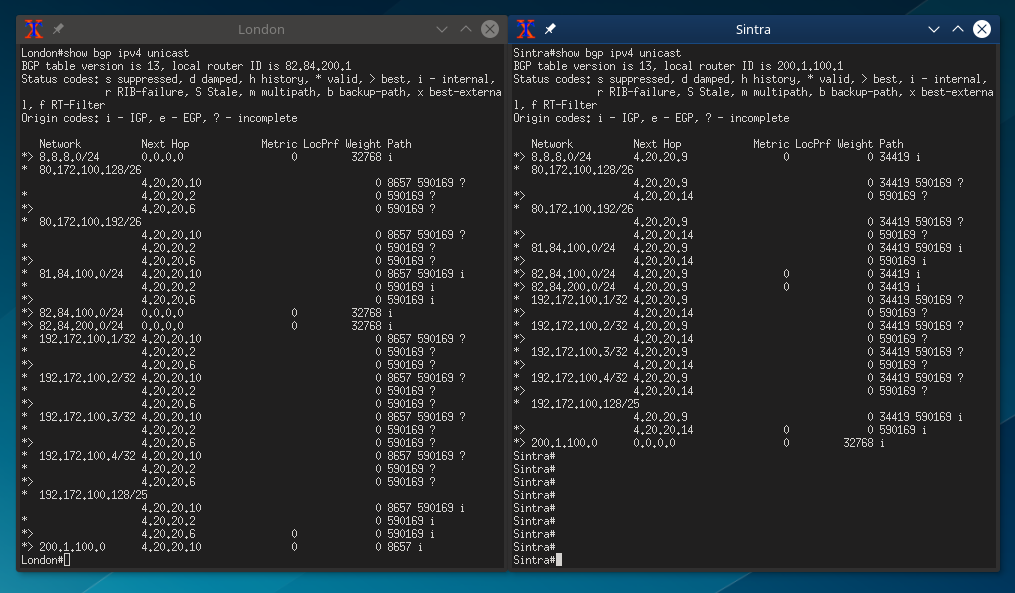
\includegraphics[width=340pt]{private_as_removal_ipv4.png}}
\caption{Remoção do AS privado em IPv4}
\label{schema}
\end{figure}

\begin{figure}[H]
\centerline{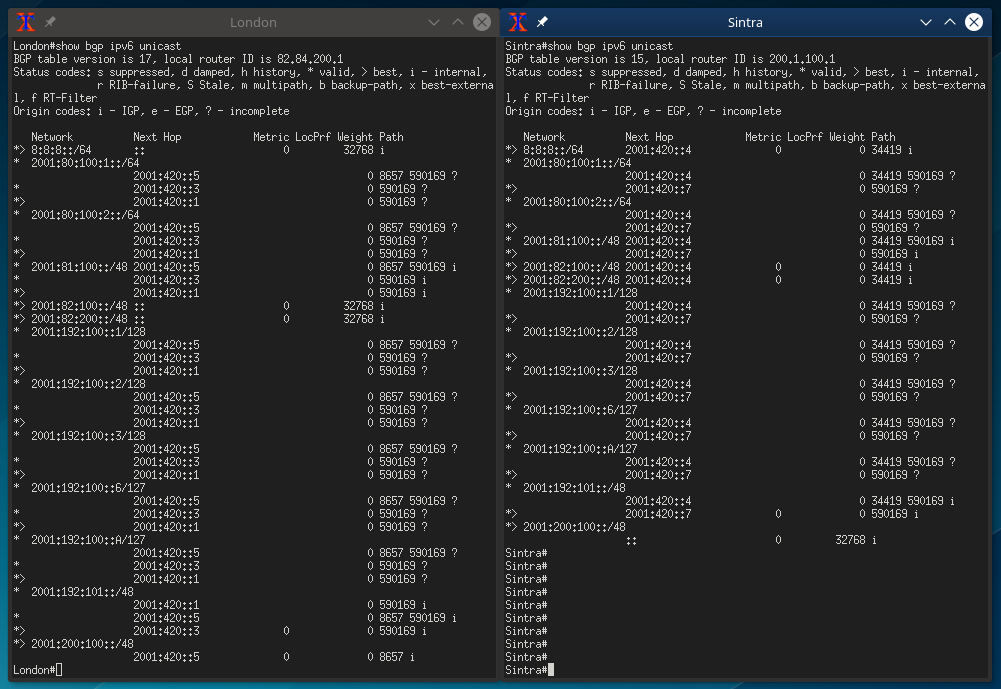
\includegraphics[width=340pt]{private_as_removal_ipv6.png}}
\caption{Remoção do AS privado em IPv6}
\label{schema}
\end{figure}


\section{Routing Constraints}

Neste projecto todas as restrições de routing apresentadas a seguir foram efectuadas usando route-map para efectuar a respectiva regra, ou negar a rota, ou aumentar a local preference da rede anunciada no iBGP.

\subsection{Internet Traffic}

``IP traffic towards Internet should be preferably routed via ISP S (Lisboa).''
\newline

Se a rota pertence à internet incrementa-se a preferência local (podia-se ter usado 0.0.0.0 para representar qualquer outra rede externa, ou seja, internet). No trecho de código seguinte podemos ver que se o ip da internet se verificar, coloca uma preferência local acima da default, caso não seja, anuncia a rota como veio.

\begin{lstlisting}[caption=Route-map para a Internet]
access-list 5 permit 8.8.8.0 0.0.0.255

route-map INTERNET_LP permit 10
 match ip address 5
 set local-preference 200

route-map INTERNET_LP permit 20
\end{lstlisting}

Como se pretende dar mais preferência à ligação entre Sintra e Lisboa quando o tráfico vai para a internet, aplica-se o route-map a todas as rotas anunciadas por Sintra a Lisboa, sendo que se alguma dessas rotas anunciadas por Sintra pertencer a internet, a preferência local será aumentada.\\

\begin{lstlisting}[caption=Route-map da Internet no Neighbor Sintra no Router de Lisboa]
router bgp 9.345
 address-family ipv4
  ...
  neighbor 4.20.20.13 route-map INTERNET_LP in
\end{lstlisting}

\subsection{Net L1 and Net L2 Preferences}

``IP traffic towards netL1 and netL2, should be preferably routed via Porto from Aveiro, and via Lisboa from Faro.''
\newline

Definiu-se a seguinte route-map em Aveiro e Faro, tendo em conta que ambos querem aumentar a preferência para a route-map na netL1 e netL2, a única diferença é por onde querer ir (só muda onde é aplicada a route-map), então definiu-se a mesma para os dois.

\begin{lstlisting}[caption=Route-map para a netL1 e netL2]
access-list 10 permit 82.84.100.0 0.0.0.255
access-list 10 permit 82.84.200.0 0.0.0.255

route-map LNET_LP permit 25
 match ip address 10
 set local-preference 210
route-map LNET_LP permit 30
\end{lstlisting}

Depois de definida a route-map, aplicou-se a rota ao neighbor respectivo.

Se Aveiro receber uma rota anunciada pelo Porto que cumpra a route-map, aumenta-lhe a perferência. Em Faro caso receba uma rota anunciada por Lisboa que cumpra a route-map, aumenta-lhe a preferência local.

Isso fez-se através do seguinte código.\\
\begin{lstlisting}[caption=Route-map LNET\_LP no Neighbor Porto no Router de Aveiro]
  neighbor 192.172.100.1 route-map LNET_LP in
\end{lstlisting}

\begin{lstlisting}[caption=Route-map LNET\_LP no Neighbor Lisboa no Router de Faro]
  neighbor 192.172.100.2 route-map LNET_LP in
\end{lstlisting}

\subsubsection{BGP IP Route - Faro e Aveiro para a rede 82.84.X.0}

Na imagem seguinte pode-se verificar que Aveiro tem uma preferencia local de 210 para a rede 82.84.100.0 e 82.84.100.0 por 192.172.100.1 (Porto) e Faro tem uma preferencia local de 210 por 192.172.100.2 (Lisboa), tal como previsto.

\begin{figure}[H]
\centerline{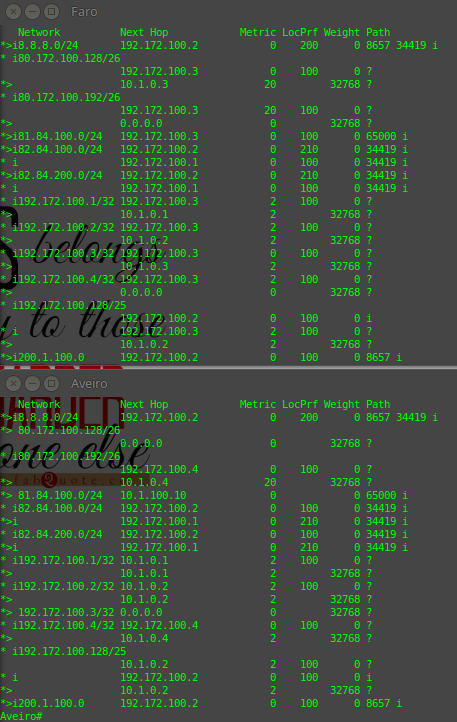
\includegraphics[width=280pt]{Selection_001.png}}
\caption{BGP IP Route - Faro e Aveiro (Local Preferences para a rede 82.84.x.0)}
\label{schema}
\end{figure}

\subsection{SIP Proxy 2 Traffic}

``IP traffic for remote SIP proxy 2 (to network netS1) should be routed only via Lisboa using the direct peering link to ISP S.''
\newline

Para fazer com que Lisboa -> Sintra fosse o único peering possível do ISP X para a NetS1, optou-se pela estratégia oposta, negar todas as saídas possíveis, ou seja, tudo o que anunciar a NetS1 e que não seja aquele link não é aceite. Sendo definida a seguinte rota:\\

\begin{lstlisting}[caption=Route-map SIP\_ROUTE para cancelar rotas]
access-list 6 permit 200.1.100.0 0.0.0.255

route-map SIP_ROUTE deny 11
 match ip address 6
route-map SIP_ROUTE permit 21
\end{lstlisting}

Sendo que foi preciso definir nos neighbors as rotas, neste caso, em Lisboa e Porto, rotas para a NetS1 recebidas pelo link de London.\\

\begin{lstlisting}[caption=Cancelar rota para NetS1 recebida em Lisboa por London]
neighbor 4.20.20.5 route-map SIP_ROUTE in
\end{lstlisting}

\begin{lstlisting}[caption=Cancelar rota para NetS1 recebida no Porto por London]
neighbor 4.20.20.1 route-map SIP_ROUTE in
\end{lstlisting}

\subsection{Non-Transit ISP-X}

Para efectuar o Non-Transit foi preciso definir uma verificação no as-path, se o AS-PATH for vazio, ou contiver apenas o AS 65000 (privado) significa que é uma rota interna e pode ser anunciada para que os outros saibam que aquele neighbor pode ser usado para chegar a rede anunciada, sendo que redes que contenham outros AS-PATH (Sistemas autonomos externos não serão anunciados para fora).\\

Teve-se de verificar para o AS 65000 porque ele atravessa pelo AS 9.345 para sair para London ou Sintra, e o rm-private-as é apenas retirado depois da validação das route-maps definidas no neighbor.\\

Sendo que se usou a seguinte route-map em todas as saídas possíveis do AS 9.345:

\begin{lstlisting}[caption=Tornar ISP X num AS Non-Transit]
ip as-path access-list 4 permit ^$
ip as-path access-list 4 permit ^65000$
route-map NON_TRANSIT permit 10
 match as-path 4
\end{lstlisting}

Sendo depois aplica-se esta route-map em Lisboa e no Porto em todos os neighbors ao anunciar rotas para fora (neighbor VIZINHO route-map NON\_TRANSIT out).

\chapter{MPLS}

\section{MPLS Tunnel for SIP Traffic}

Para o SIP Traffic é importante a existência de Tuneis entre as empresas e o SIP Proxy, sendo que definiu-se que o Tunnel em Aveiro até Lisboa seria suficiente, porque as ligações de Aveiro a empA1 é uma ligação ponto-a-ponto e Aveiro é que pertence ao Core do ISP (também podemos verificar que o limite do iBGP só chega até Aveiro, a empA1 já não tem BGP), daí termos escolhido Aveiro como um dos extremos do túnel, o mesmo se verifica para Faro.\\

\begin{figure}[H]
\centerline{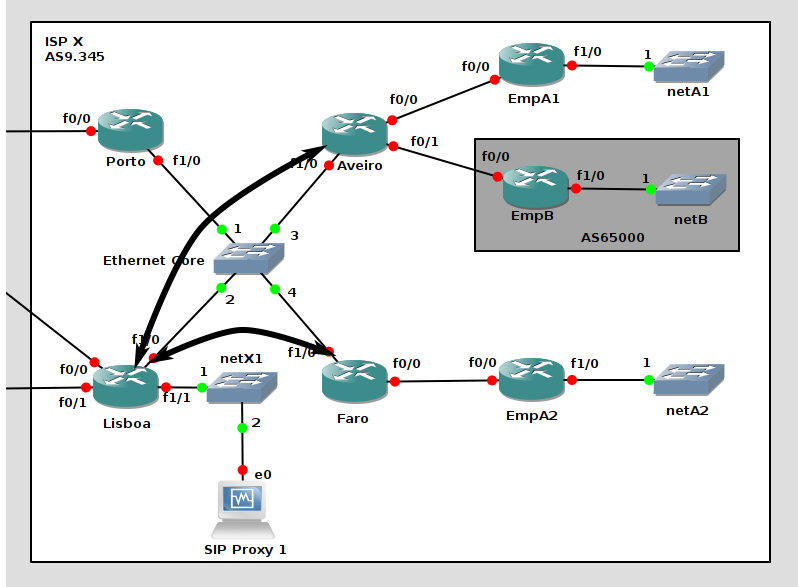
\includegraphics[width=300pt]{network_tunnel.png}}
\caption{MPLS Tunnel entre SIP Proxy 1 e Aveiro (empA1 e EmpB) e o SIP Proxy e Faro (empA2)}
\label{schema}
\end{figure}


Sendo assim criou-se dois túneis, um túnel (1) para fazer a transição do tráfico da Empresa A1 (ramo de Aveiro) e da Empresa B até ao SIP Proxy 1 e vice-versa. Depois criou-se outro túnel para o ramo da Empresa A em Faro (empA2) até ao SIP Proxy 1. Tal como mostra a imagem anterior.\\

De forma a activar o MPLS com RSVP-TE sobre a rede entre Aveiro/Faro e Lisboa foi preciso activar na configuração OSPF de forma a ele se propagar (Loopbacks e OSPF já estavam definidos anteriormente, foi só activar o MPLS traffic engineering), usando o seguinte comando (em todas as interfaces físicas e na configuração geral do router, isto entre Aveiro/Faro e Lisboa):\\

\begin{lstlisting}[caption=MPLS Tunnel - Activar MPLS TE no OSPF]
 mpls traffic-eng area 0
 mpls traffic-eng router-id Loopback 0
\end{lstlisting}

Para activar o RSVP ainda é preciso definir a largura de banda do RSVP, tendo em conta que ambos os túneis vão usar o mesmo RSVP e pretende-se 1Mbits em cada túnel MPLS, é preciso definir no mínimo 2Mbits na largura de banda RSVP para ter os dois túneis activos ao mesmo tempo, no entanto definiu-se 8Mbits para se ter uma pequena margem. Usando assim o seguinte comando nas interfaces fisicas.\\

\begin{lstlisting}[caption=MPLS Tunnel - Activar RSVP]
ip rsvp bandwidth 8096 8096
\end{lstlisting}

Para configurar o Túnel em Aveiro usou-se a seguinte sequência de comandos:\\
\begin{lstlisting}[caption=MPLS Tunnel - Aveiro]
interface Tunnel1
 ip unnumbered Loopback0
 tunnel mode mpls traffic-eng
 tunnel destination 192.172.100.2
 tunnel mpls traffic-eng bandwidth 1024
 tunnel mpls traffic-eng path-option 1 dynamic
\end{lstlisting}

Sendo que em Lisboa foi definido um Túnel para Aveiro também com a respectiva interface de Loopback de Aveiro, o mesmo foi efectuado para Faro.\\

Depois de ter definido todas as interfaces e activar correctamente o MPLS com RSVP, é preciso indicar como é que é possível entrar no túnel. Sendo que foi definido o seguinte código no router de Lisboa para permitir a entrada no túnel:\\

\begin{lstlisting}[caption=MPLS Tunnel - Lisboa rota de entrada no túnel]
interface FastEthernet1/1 	!interface do SIP Proxy 1
 ip policy route-map SIP_PORT

route-map SIP_PORT permit 12                 !Aveiro
 match ip address VoIP-TRAFFIC 7             !SIP e ACL7
 set interface Tunnel1              

route-map SIP_PORT permit 13                 !Faro
 match ip address VoIP-TRAFFIC 8             !SIP e ACL 8
 set interface Tunnel2

access-list 7 permit 10.1.1.0 0.0.0.127      !EmpA1
access-list 7 permit 81.84.100.0 0.0.0.255   !EmpB
access-list 8 permit 10.1.1.128 0.0.0.127    !EmpA2

ip access-list extended VoIP-TRAFFIC
 permit udp any any range 16384 32767
 permit udp any range 16384 32767 any
 permit udp any any eq 5060
 permit tcp any any eq 5060
 permit udp any eq 5060 any
 permit tcp any eq 5060 any
 permit udp any any eq 5061
 permit tcp any any eq 5061
 permit udp any eq 5061 any
 permit tcp any eq 5061 any
\end{lstlisting}

Este route-map é aplicado na interface que está do lado do SIP Proxy 1, ou seja, só o tráfico que vem daquela interface com destino as redes das empresas e com um porto de tráfico VoIP é que consegue atravessar por dentro do túnel, caso contrário, consegue comunicar mas não por dentro do túnel (acabando por perder os seus benefícios).\\

Do lado de Aveiro/Faro foi preciso fazer uma configuração similar para entrar no túnel, no entanto não se verificou o IP destino, desde que seja SIP entra pelo túnel:

\begin{lstlisting}[caption=MPLS Tunnel - Aveiro rota de entrada no túnel]
interface FastEthernet0/0                  !Empresa A1
 ip vrf forwarding VPN-ClientA
 ip address 10.1.100.1 255.255.255.252
 ip policy route-map SIP_PORT

interface FastEthernet0/1                  !Empresa B
 ip address 10.1.100.9 255.255.255.252
 ip policy route-map SIP_PORT

route-map SIP_PORT permit 11
 match ip address VoIP-TRAFFIC
 set interface Tunnel1
\end{lstlisting}

Em Faro foi feito uma configuração similar a de Aveiro, sendo isto o necessário para ter ambos os túneis a funcionar correctamente e em simultâneo.

\subsection{Validação do Túnel}

A validação deste túnel não pode ser feita através de GNS3 (pelo menos totalmente) porque não se via nenhum label MPLS o que está correcto, Lisboa é o penultimo router do Tunnel para Aveiro, logo é suposto ser o último pop do label.\\

Para confirmar que de facto estava a entrar dentro do tunnel usou o comando: show interfaces Tunnel 1\\

E verificou-se o estado do Túnel como também o número de pacotes que tinham lá passado, após verificar o número de pacotes efectuou-se um ping com um VPCS (são os unicos que permitem pings usando UDP e o porto) no porto 5060 em UDP e verificou-se que ao efectuar show interfaces Tunnel 1 novamente, o número de pacotes que tinha atravessado o túnel tinha sido 5.\\

A imagem seguinte mostra a validação efectuada, sendo 93 o número de pacotes inicial e 98 após o envio de pacotes UDP para a network da empresa A.\\

\begin{figure}[H]
\centerline{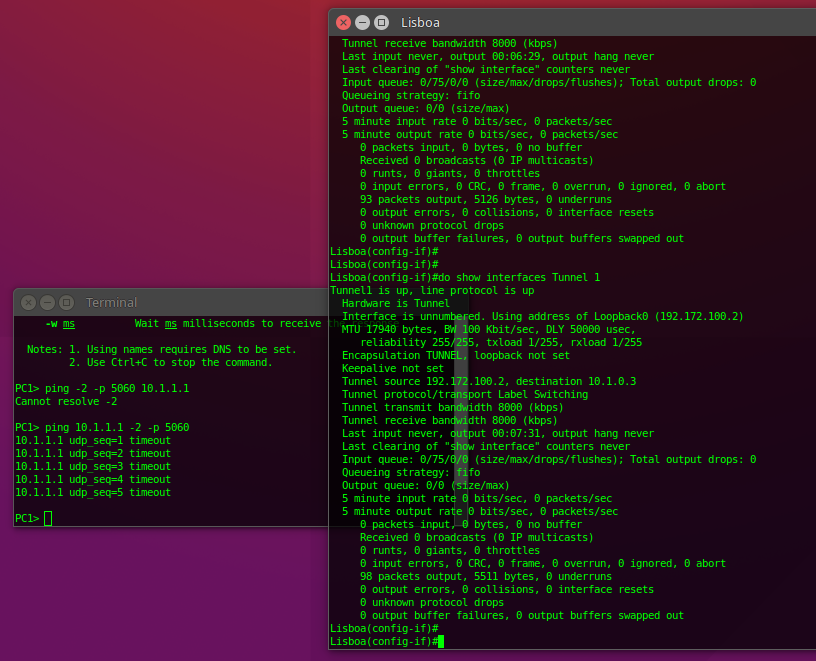
\includegraphics[width=300pt]{tunnel_mpls.png}}
\caption{MPLS Tunnel - Teste de VPCS em Lisboa para interface da EmpA1 (Pacote UDP)}
\label{schema}
\end{figure}

\section{MPLS VPN}

\subsection{Internal Connectivity}
Para configurar a VPN é preciso criar uma VRF que é o que vai permitir ter um encaminhamento especifico para a network da empresa A, neste caso vai ter um routing table específica para a rede da empresa A, sendo esse o panel da VRF (Routing e Forwarding).\\

Para além disso cada VRF tem de ter um identificador que a permite destinguir de outras VRF existentes (neste caso só existe a da empresa A), e é preciso indicar que todas as rotas desta VRF serão exportadas por VRF com o mesmo identificador e também irá importar rotas de VRFs com o mesmo identificador. Sendo assim definida a seguinte VRF:\\

\begin{lstlisting}[caption=VPN - Criar uma VRF e associar um router distinguisher]
ip vrf VPN-ClientA
 rd 9345:1
 route-target export 9345:1
 route-target import 9345:1
\end{lstlisting}

Depois de definir a VRF é preciso indicar a interface a qual a VRF estará associada, neste caso será na interface FastEthernet0/0 em Aveiro e FastEthernet0/0 em Faro sendo a outra ponta.

\begin{lstlisting}[caption=VPN - Associar a VRF a uma interface]
interface FastEthernet0/0
 ip vrf forwarding VPN-ClientA
\end{lstlisting}


Para além disso é preciso identificar aos Provider Edge (PE), neste caso, Aveiro e Faro, quais são os pacotes que pertencem as VPNs, para isso efectua-se o seguinte comando.\\

\begin{lstlisting}[caption=VPN - Anunciar os labels das VPNs]
router bgp 9.345
 address-family vpnv4
  neighbor 192.172.100.4 activate
  neighbor 192.172.100.4 send-community both
 address-family ipv4 vrf VPN-ClientA
  redistribute connected
\end{lstlisting}

Após efectuar este pequeno comando reparou-se que apenas se tinha ligação entre a rede directamente ligada a Aveiro e a rede directamente ligada a Faro, com a VPN a funcionar apesar de tudo. Isto deve-se a VRF estar completamente vazia apenas com as directamente ligadas!\\

O que se fez para resolver este problema e ter conectividade não só com a rede directamente ligada a Aveiro mas também com a rede da Empresa A1 e da Empresa A2 foi activar um processo OSPF na VRF como mostra a imagem seguinte rodeado com circulos pretos:\\

\begin{figure}[H]
\centerline{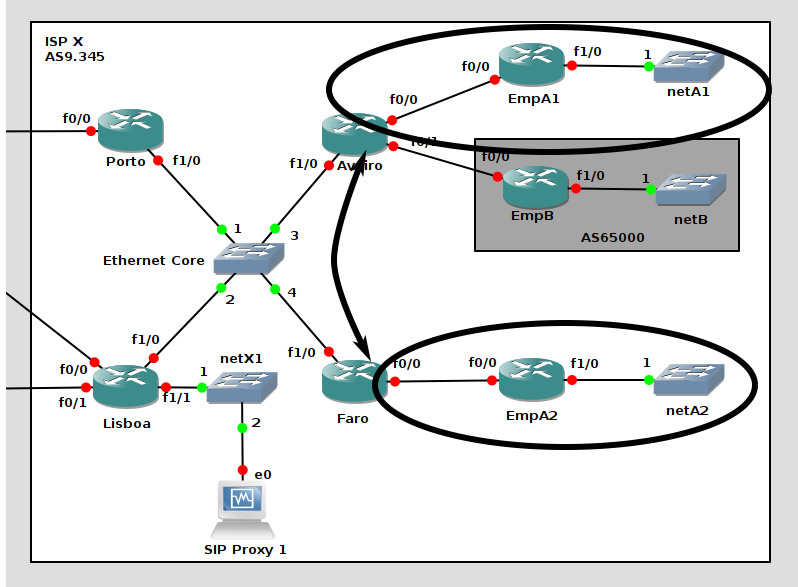
\includegraphics[width=300pt]{network_vpn.png}}
\caption{MPLS VPN entre Aveiro e Faro (empresas A1 e A2)}
\label{schema}
\end{figure}

Para activar o OSPF na VRF foi preciso executar os seguintes comandos:\\

\begin{lstlisting}[caption=VPN - Suporte de OSPF entre o PE e o CE]
router ospf 200 vrf VPN-ClientA
 network 10.1.0.0 0.0.255.255 area 0
\end{lstlisting}

Depois de activar OSPF na VRF do router de Aveiro, Faro, EmpA1 e EmpA2 passou-se a ter total conectividade dentro da VPN.

\subsection{External Connectivity}

Para obter conectividade externa é preciso indicar a rede da VPN como sair para fora da rede interna, neste caso faz-se com uma rota estática (que é distribuida pelo OSPF da VRF) definida na VRF indicando a interface de saída.\\

\begin{lstlisting}[caption=VPN - Rota de saída da VPN-ClientA]
ip route vrf VPN-ClientA 0.0.0.0 0.0.0.0 192.172.100.1 global
\end{lstlisting}

E é preciso indicar às redes de fora (ou seja, a todo o iBGP e eBGP) quais são as redes que estão disponiveis dentro da VRF.\\

\begin{lstlisting}[caption=VPN - Anunciar rotas disponiveis dentro da VPN do lado de Aveiro]
ip route 10.1.1.0 255.255.255.128 FastEthernet0/0
ip route 80.172.100.128 255.255.255.192 FastEthernet0/0
\end{lstlisting}

Sendo estas rotas distribuidas para o OSPF para funcionar na rede de interna, e para o BGP para funcionar externamente de igual forma, existindo assim tanto conectividade dentro da VPN como de fora para dentro e vice-versa.

\chapter{VoIP SIP}

Neste projeto foi pedido que existisse um serviço de SIP-VoIP para todos os clientes empresariais do ISP X. Esse serviço VoIP deve fornecer conetividade entre todos os clientes empresariais, bem como fornecer compatibilidade com chamadas oriundas de PTSN, encaminhadas pelo SIP Proxy 2. O serviço de VoIP deve também encaminhar as chamadas para redes externas utilizando o SIP Proxy 2.

\section{Internal Extensions}

A configuração dos clientes é a seguinte:

\begin{lstlisting}[caption=SIP Proxy 1 - /etc/asterisk/sip.conf]
[EmpA1]
type=friend
host=dynamic
secret=labcom
context=phones
allow=all

[EmpA2]
type=friend
host=dynamic
secret=labcom
context=phones
allow=all

[EmpB]
type=friend
host=dynamic
secret=labcom
context=phones
allow=all
\end{lstlisting}

Apenas existe uma conta por empresa, para ser possível testar a conetividade entre elas. Na realidade poderiam existir muitas mais sem que existem problemas.\\

De seguida configurou-se a extensões dos clientes, sendo elas:

\begin{lstlisting}[caption=SIP Proxy 1 - /etc/asterisk/extensions.conf]
[phones]
exten => 1000,1,Answer(500)
exten => 1000,2,PlayBack(demo-congrats)
exten => 1000,3,PlayBack(vm-goodbye)
exten => 1000,4,HangUp()

exten => 2000,1,Dial(SIP/EmpA1)
exten => 2000,2,voicemail(3000@corporations_voicemail)
exten => 2000,3,PlayBack(vm-goodbye)
exten => 2000,4,HangUp()

exten => 2001,1,Dial(SIP/EmpA2)
exten => 2001,2,voicemail(3001@corporations_voicemail)
exten => 2001,3,PlayBack(vm-goodbye)
exten => 2001,4,HangUp()

exten => 2002,1,Dial(SIP/EmpB)
exten => 2002,2,voicemail(3002@corporations_voicemail)
exten => 2002,3,PlayBack(vm-goodbye)
exten => 2002,4,HangUp()

exten => 3000,1,voicemail(3000@corporations_voicemail)
exten => 3001,1,voicemail(3001@corporations_voicemail)
exten => 3002,1,voicemail(3002@corporations_voicemail)
\end{lstlisting}

A extensão 1000 serve para testar a conetividade com o servidor. 
A extensão 2000 é a extensão do polo 1 da empresa A. 
A extensão 2001 é a extensão do polo 2 da empresa A. 
A extensão 2002 é a extensão da empresa B. 
As extensões 3000, 3001 e 3002 dão acesso ao voicemail das empresas.
Todas as extensões 2000, 2001 e 2002 caso estejam ocupadas vão parar ao voicemail.\\

As configurações do voicemail são as seguintes:

\begin{lstlisting}[caption=SIP Proxy 1 - /etc/asterisk/voicemail.conf]
[corporations_voicemail]
3000 => 1212,EmpA1
3001 => 1212,EmpA2
3002 => 1212,EmpB
\end{lstlisting}


\section{PTSN Calls Support}

As chamadas provenientes da rede PTSN vão utilizar a seguinte configuração para serem reencaminhadas para as respetivas empresas.

\begin{lstlisting}[caption=SIP Proxy 1 - /etc/asterisk/extensions.conf]
[phones]
...
exten => _2341000XX,1,Dial(SIP/EmpA1)
exten => _2341000XX,2,voicemail(3000@corporations_voicemail)
exten => _2341000XX,3,PlayBack(vm-goodbye)
exten => _2341000XX,4,HangUp()

exten => _2891001XX,1,Dial(SIP/EmpA2)
exten => _2891001XX,2,voicemail(3001@corporations_voicemail)
exten => _2891001XX,3,PlayBack(vm-goodbye)
exten => _2891001XX,4,HangUp()

exten => _2341002XX,1,Dial(SIP/EmpB)
exten => _2341002XX,2,voicemail(3002@corporations_voicemail)
exten => _2341002XX,3,PlayBack(vm-goodbye)
exten => _2341002XX,4,HangUp()
\end{lstlisting}

O underscore indica o inicio do padrão que queremos utilizar e o X indica números de 0 a 9. De resto a configuração é semelhante a anterior.

\section{Forward to SIP Proxy 2}

Para fazer reencaminhar as chamadas VoIP para redes externas é preciso alterar as configurações dos dois servidores SIP.

\begin{lstlisting}[caption=SIP Proxy 1 - /etc/asterisk/sip.conf]
...
[Server2]
type=peer
host=200.1.100.2
secret=labcom
username=Server1
\end{lstlisting}

\begin{lstlisting}[caption=SIP Proxy 2 - /etc/asterisk/sip.conf]
[Server1]
type=peer
host=192.172.100.130
secret=labcom
context=phones
\end{lstlisting}

\begin{lstlisting}[caption=SIP Proxy 1 - /etc/asterisk/extensions.conf]
...
exten => _X!,1,Dial(SIP/${EXTEN}@Server2,10)
exten => _X!,2,HangUp()
\end{lstlisting}

\begin{lstlisting}[caption=SIP Proxy 2 - /etc/asterisk/extensions.conf]
[phones]
exten => _X!,1,Answer(500)
exten => _X!,2,PlayBack(demo-congrats)
exten => _X!,3,PlayBack(vm-goodbye)
exten => _X!,4,HangUp()
\end{lstlisting}

No servidor 1 foi preciso criar um peer para permitir que o mesmo se consiga ligar ao servidor 2. Foi também preciso criar uma nova regra nas extensões do servidor 1 que reencaminhe todas as chamadas VoIP com destino em extensões externas para o servidor 2, assim sendo foi criado o padrão \_X!, onde o underscore indica o inicio do padrão, o X indica qualquer número e o ! todas as extensões não definidas anteriormente. Caso se encontre alguma chamada para uma extensão deste tipo, o servidor 1 deve fazer uma SIP URI dial para o servidor 2 para onde envia a extensão.\\
No servidor 2 foi preciso criar um peer para indicar que o servidor 1 se vai ligar a ele. As extensões são idênticas às definidas anteriormente.

\listoffigures
\lstlistoflistings
\bibliographystyle{plain}
\bibliography{proj2}

\end{document}
